\chapter{Introduction}
The goal of this chapter is to give an overview of the available knowledge about stearoyl-CoA desaturase (SCD1) which is the main focus of this thesis. SCD1 is an iron-containing enzyme and member of the large non-heme iron enzyme family. The chapter starts  explaining the role of iron in biological systems and moves on to discuss the experimental and theoretical methods used to study non-heme iron enzymes. An overview of the rich chemistry of both binuclear and mononuclear non-heme iron enzymes is given before discussing the reactivity and importance of SCD1.

\section{Role of iron in biological systems}
Iron is the fourth most abundant element on Earth, comprising the majority of the Earth's core \cite{inorganic_chemistry_book}. Commercially, it is mostly used for steel production. Iron oxides are important polishing agents and pigments. Iron can exist in oxidation states between +2 and +6, with +2 and +3 being the most common. Depending on the ion's coordination environment, different spin states are possible. Iron's natural abundance and electronic state versatility probably explain why it is heavily utilized by biological systems for the transport of oxygen, electron transport, and catalysis \cite{Frey2012}.

Iron is an essential trace element for all organisms. An average human contains around 4.2 grams of iron. The majority of it is stored in the liver, spleen and bone marrow in the form of the metalloprotein \textit{ferritin}. It consists of 24 identical subunits forming a cavity inside of which several thousand iron atoms can be stored in the form of iron oxides \cite{Harrison1996}. Active ions are mostly part of protein prosthetic groups. The most common iron-containing prosthetic group is the heme group. It consists of an iron ion coordinated by a planar tetradentate porphyrin ring \cite{Lehninger}. In hemoglobin and myoglobin, proteins important for transport and storage of oxygen, there is an additional histidine ligand. O\textsubscript{2} binds to the remaining free coordination position trans to the histidine. O\textsubscript{2} binding oxidises the high-spin Fe$^{\mathrm{II}}$ center to low-spin Fe$^{\mathrm{III}}$ which reduces O\textsubscript{2} to a superoxo [O\textsubscript{2}]$^{-}$ ligand. Heme-containing proteins also act as catalysts. Cytochromes P-450 catalyze the monooxygenation of aromatic and aliphatic C-H bonds to C-OH \cite{Denisov2005}. The active site contains a heme group where a low-spin Fe$^{\mathrm{III}}$ ion forms a covalent bond with a cysteine sulfur. The active species is high-valent Fe$^{\mathrm{IV}}$=O whose formation is accompanied with a one-electron oxidation of the porphyrin ring.

Iron-sulfur proteins are another big group of iron-containing proteins. All of them contain iron-sulfur clusters made up of high-spin Fe$^{\mathrm{II}}$ and Fe$^{\mathrm{III}}$ centres coordinated by four sulfur ligands, either free sulfide ions or cystein sulfurs \cite{inorganic_chemistry_book}. Rubredoxins contain only one FeS\textsubscript{4} unit while ferredoxins contain several connected units. They facilitate electron transport processes with the interconversion of Fe$^{\mathrm{II}}$ and Fe$^{\mathrm{III}}$. Different compositions of the Fe$_x$S$_y$ cluster and changes in the protein environment enable iron-sulfur proteins to adapt a wide range of reduction potentials.

The final large group are non-heme iron-containing proteins \cite{Solomon2000}. The majority of proteins in this group catalyze oxygen-mediated oxidation  reactions. O\textsubscript{2} in its triplet ground state is inert towards singlet organic substrates. Non-heme iron (NHFe) enzymes activate O\textsubscript{2} by converting it to more reactive iron-oxygen species, e.g., iron-superoxo, iron-peroxo, iron-oxo, and various oxygen bridged diiron species. Based on the structure of the active site they can be divided into mononuclear and binuclear enzymes. 


\section{Non-heme iron enzymes}
Oxygen activation enables NHFe enzymes to catalyze a variety of chemical reactions: desaturation, halogenation, oxygenation, hydroxylation, aromatic ring cleavage and many more \cite{Solomon2016,Jasniewski2018}. The reactions are usually highly selective and it is remarkable that only a couple of reactive iron-oxygen species are responsible for all the transformations (see below). This implies that the rest of the protein environment is crucial for fine-tuning its activity. NHFe enzymes are interesting from an industrial perspective because of their ability to activate inert aliphatic and aromatic C-H bonds \cite{Shilov1997}. Understanding the factors controlling their reactivity potentially enables design of new catalysts from readily available iron. Some NHFe enzymes are potential drug targets. For example, stearoyl-CoA desaturase (SCD1), an important enzyme in fatty acid metabolism, is an exciting target for the development of novel diabetes and anticancer drugs \cite{Dobrzyn2005,Gaszewska2019}.


\subsection{Experimental and theoretical approaches for the study of NHFe enzymes}
The iron ion in NHFe enzymes is usually coordinated by weak-field nitrogen or oxygen ligands, e.g., the imidazole side chain of histidine, water, hydroxide, carboxylates... They are harder to study than heme enzymes \cite{Solomon2003}. The porphyrin ring simplifies the possible coordination environments by leaving only two free coordination positions, while porphyrin's characteristic $\pi \rightarrow \pi^{*}$ transitions enable simple spectroscopic characterisation. NHFe$^{\mathrm{II}}$ sites usually lack ligand to metal charge transfer transitions and are not detectable by electron paramagnetic resonance (EPR) spectroscopy. However, they do possess iron $d \rightarrow d$ transitions in the near-infrared region which are characteristic of the coordination environment. Those transitions are low intensity in absorption spectroscopy, but intense in magnetic circular dichromism (MCD) spectroscopy. M\"ossbauer spectroscopy can be used to determine the oxidation and spin state of iron ions and for gaining information about the symmetry of the ligand field around them \cite{Crichton2016_essential_role_iron}. Structural information about the iron site can be obtained  with the extended X-ray absorption fine structure (EXAFS) technique \cite{Feiters2013}. It usually requires comparing the results with spectra of smaller synthetic complexes or metalloproteins of known structure. The advantage is that no crystal sample of the protein is required and higher accuracy than with X-ray crystallography is possible.

Detecting short-lived intermediates is an advantage of spectroscopic techniques over X-ray crystallography. To deduce the molecular structure of those species, it is usually necessary to correlate the spectroscopic data with theoretical quantum mechanical (QM) calculations and results for smaller synthetic iron complexes of known geometry \cite{Rokob2016}. The properties which made iron desirable in biology present a challenge for QM calculations. The variety of possible electronic states results in a large multireference character of NHFe sites. This is especially problematic for the binuclear sites which exhibit spin coupling between the two iron ions. Another problem is the size of the active sites. A system of a single iron ion coordinated with 6 imidazole ligands, mimicking histidines, already contains 55 atoms. This means that most active sites are too large for the ``gold standard'' methods usually used for smaller molecules, like coupled cluster with singles, doubles, and perturbative triples [CCSD(T)]. Because of this, density functional (DFT) methods are most commonly used, even though they can struggle with multiconfigurational systems. A lack of a reliable reference method means that the selection of the DFT functional is not clear. One approach is to benchmark the functionals against experimental spectroscopic results \cite{Rokob2016}. The complete active space self-consistent field method (CASSCF) is a multireference method able to describe multiconfigurational systems, but it suffers from exponential scaling with respect to the number of active space orbitals. The density matrix renormalization group (DMRG) method significantly increases the maximum number of active orbitals, but there is no systematic way of selecting them. 

Besides selecting the QM method, we need to decide how to model the active site. Cluster models consider only the isolated active site, while hybrid quantum mechanics/molecular mechanics (QM/MM) considers the whole protein in a model where the active site is described with QM and the rest of the system with MM \cite{Blomberg2014}. Cluster models are more popular because they are cheaper and easier to set up, but errors can occur: if some important residues are not included, if the active site is very flexible or if explicit solvent molecules participate in the reaction. QM/MM models describe more accurately the steric constraints of the active site and can model the participation of solvent molecules. Furthermore, once the QM/MM system is created, it is very easy to initiate molecular dynamics (MD) simulations to explore different conformations of the system. In many cases the rest of the environment is essential to correctly describe the reactivity of NHFe enzymes. A QM/MM study of initial oxygen binding to the NHFe center of histone demethylase showed that residues in the extended protein environment, not directly bound to the active site, are crucial for stabilizing the iron(III)-superoxo complex \cite{Cortopassi2015}. Du and coworkers showed the importance of water molecules in controlling the reactivity of 2-hydroxyethylphosphonate dioxygenase (HEPD) \cite{Du2012}. MD simulations on isopenicillin N synthase (IPNS) suggest that dynamical effects of the protein environment reduce the O$-$O bond breaking barrier by several kcal/mol \cite{Kawatsu2011}. 


\subsection{Dioxygen activation in mononuclear NHFe enzymes}
Even though mononuclear NHFe enzymes catalyze diverse reactions, they share a common strategy for dioxygen activation (Fig.\,\ref{fig:NHFe_O2}) \cite{Ray2014}. The figure does not show elementary reaction steps but rather general pathways to active intermediates observed or suggested for mononuclear NHFe enzymes. The exact way of reaching each intermediate differs from enzyme to enzyme and the reaction does not need to go all the way to the iron-oxo species. The elementary reaction steps are usually not well understood due to the intermediates' short lifetime, so quantum chemical methods are essential for understanding the whole reaction mechanism. The first step is usually binding of O\textsubscript{2} to Fe$^{\mathrm{II}}$ and formation of an iron(III)-superoxo species. Subsequent one-electron reduction forms an iron(III)-peroxo species. Protonation of iron(III)-peroxo, or hydrogen atom transfer to iron(III)-superoxo, leads to iron(III)-hydroperoxo which can undergo homolytic O$-$O bond cleavage to afford the high-valent iron(IV)-oxo species. The formed active intermediates can react in different ways with hydrogen atom abstraction (HAA) being the most common for many mononuclear enzymes. After HAA the mechanism can branch out towards desaturation, halogenation, hydroxylation or ring closure.

\begin{figure}[htbp]
    \centering
    
\includegraphics[width=0.8\textwidth]{Figures/Dioxygen_NHFe.pdf}
    \caption{General strategy for dioxygen activation by mononuclear non-heme iron enzymes. Adapted from \cite{Ray2014}.}
    \label{fig:NHFe_O2}
\end{figure}

The most common and best understood active species is iron(IV)-oxo. It has been trapped and characterized in synthetic biomimetic complexes \cite{Visser2013} in addition to being confirmed as the active species of many enzymes, e.g., tyrosine hydroxylase \cite{Eser2007} and taurine dioxygenase \cite{Gelasco2004}. The high-spin $S=2$ state is the ground state in mononuclear NHFe enzymes, whereas the $S=1$ state is found in heme iron(IV)-oxo species and synthetic complexes. A B3LYP cluster study suggests that the nature of the species performing HAA is best described as an iron(III)-oxyl radical \cite{Ye2011}. Theoretical studies show that HAA in the $S=1$ state proceeds only through a $\pi$ channel requiring perpendicular approach of the C-H bond to the iron(IV)-oxo bond \cite{Decker2007}. On the other hand, the $S=2$ state has both $\pi$ and $\sigma$ channels available.  

The iron(III)-superoxo species is suggested to perform HAA in the mononuclear NHFe enzyme IPNS \cite{Brown2007}, but a DFT study showed that it is in general less reactive than iron(IV)-oxo \cite{Chung2011}. No examples of HAA reactions performed by mononuclear iron(III)-peroxo species are known, while iron(III)-hydroperoxo is suggested as the active species in HAA from DNA by the anticancer drug bleomycin \cite{Chow2008}. An experimental study showed that both low- and high-spin synthetic iron(III)-hydroperoxo species are able to perform HAA \cite{Liu2013}.
 

\subsection{Dioxygen activation in binuclear NHFe enzymes}
The chemistry becomes more complex and challenging in the case of diiron sites. Binuclear NHFe enzymes can be further divided into two families: soluble and transmembrane enzymes. Significantly more is known about soluble enzymes, presumably because of the challenging nature of transmembrane proteins. X-ray diffraction experiments show that diiron sites in soluble enzymes contain a coordination environment rich in bridging carboxylate ligands with an iron-iron distance between 2.7 and 4.1 Å \cite{Jasniewski2018}. The resting state is in most cases an antiferromagnetically coupled high-spin Fe$^{\mathrm{II}}_{2}$ site. The presence of two iron centers, together with different coordination environments, results in diverse dioxygen activation mechanisms. Still, a common step for all of them is the step-wise reduction of dioxygen by electrons from iron ions. Figure \ref{fig:NHFe2_strategy} shows some of the most common reactive species and a general strategy for reaching them. We can see that they differ from species found in mononuclear enzymes in the fact that they are bridged iron-oxygen complexes.

\begin{figure}[htbp]
    \centering
    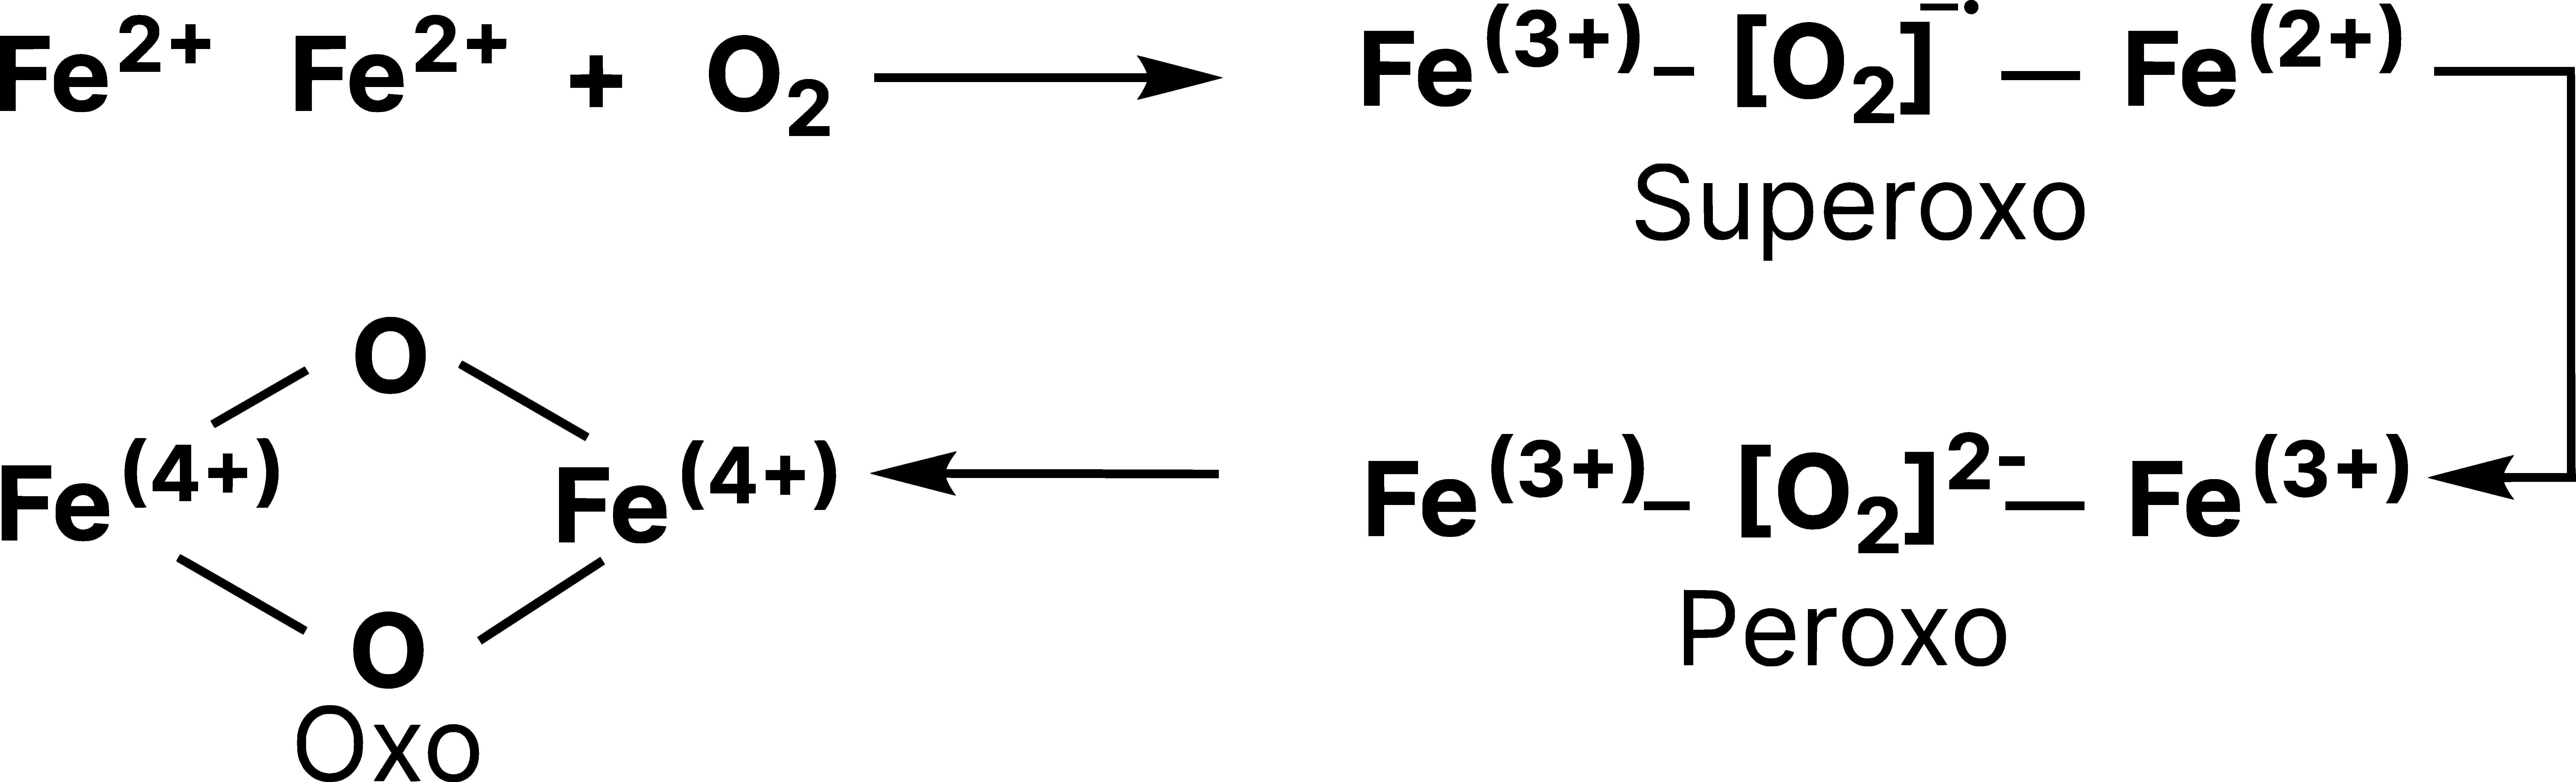
\includegraphics[width=0.7\textwidth]{Figures/Dioxygen_NHFe2.pdf}
    \caption{General strategy for dioxygen activation by soluble binucelar non-heme iron enzymes. Adapted from \cite{Ray2014}.}
    \label{fig:NHFe2_strategy}
\end{figure}

On the other hand, the diiron site in transmembrane enzymes is completely different. Strong evidence for this are the determined crystal structures of mouse and human stearoyl-CoA desaturase \cite{Bai2015,Wang2015}. One iron ion is coordinated by 5 histidine residues and the other with 4 histidines and one water molecule. The iron ions are separated by more than 6 Å, much larger than in soluble enzymes. This is possibly explained by the lack of carboxylate bridging ligands. Other representative members of this family are the alkane $\omega$-hydroxylase (AlkB) and xylene monooxygenase. Sequence comparisons showed that the coordinating histidines are conserved among all the members of the family \cite{Shanklin1994}. This can also be seen by comparing the predicted AlphaFold structures of AlkB and xylene monooxygenase with the crystal structure of SCD1 \cite{Varadi2022}. Furthermore, Chain et~al.~recently published a cryo-electron microscopy structure of AlkB from \textit{Fontimonas thermophila} fused with its electron donor protein \cite{Chai2023}. It shows the same nine histidine diiron site as in SCD1 but with a glutamate coordinated to one iron ion instead of a water molecule (Fig. \ref{fig:AlkB_structure}). The iron-iron distance is 6.1 Å. The large iron-iron distance in transmembrane enzymes possibly prohibits the formation of bridged iron-oxygen complexes and implies a completely different dioxygen activation mechanism compared to soluble enzymes. This claim must be tested because M\"ossbauer spectroscopy data on AlkB suggests the formation of bridged oxo complexes \cite{Shanklin1997}. This would require a reduction of the iron-iron distance by several Å~\cite{Shu1997}.

\begin{figure}[htbp]
    \centering
    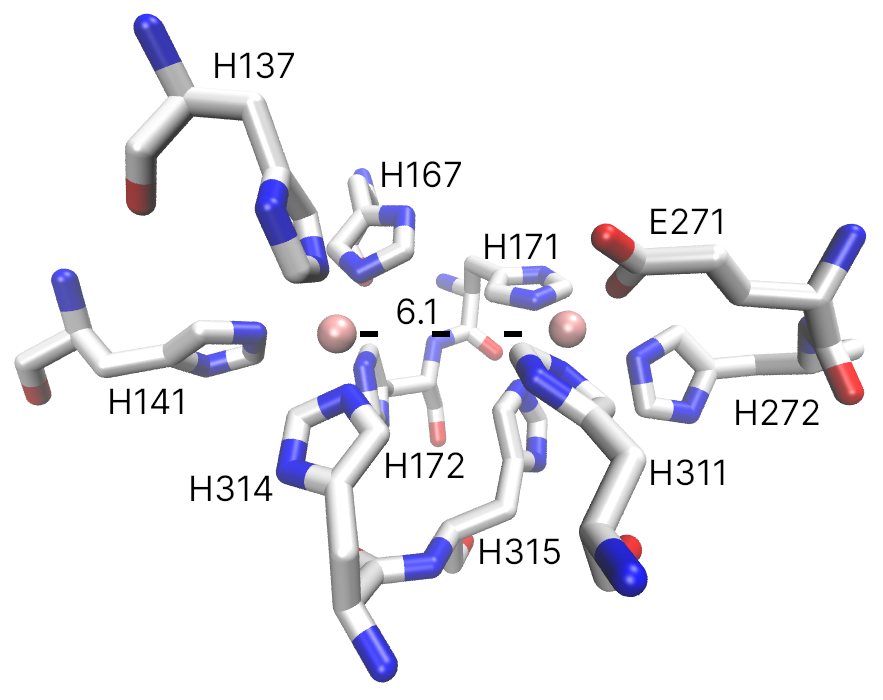
\includegraphics[width=0.7\textwidth]{Figures/8f6t.png}
    \caption{Structure of the active site of alkane $\omega$-hydroxylase (AlkB) determined by cryo-electron microscopy with 2.76 Å resolution (PDB: 8F6T, \cite{Chai2023}). Residues are shown as sticks. Distance is shown in Å. Colours: pink, iron; red, oxygen; blue, nitrogen; white, carbon.}
    \label{fig:AlkB_structure}
\end{figure}


\section{Stearoyl-CoA desaturase}
Fatty acids are carboxylic acids with a 4 to 36 carbon long, usually linear, aliphatic chain \cite{Lehninger}. They are the main component of biological membranes and play an important role in energy storage and signalling. Based on the degree of saturation we divide them into: saturated, monounsaturated, and polyunsaturated fatty acids. Because of this, it is common to name unbranched fatty acids by only specifying the number of carbon atoms and the number of double bonds. The positions of the double bonds are indicated in the superscript of $\Delta$. Following this naming convention, stearic acid is named 18:0 because it is an 18 carbon saturated fatty acid. Similarly, oleic acid is 18:1($\Delta^{9}$) because it has one double bond after carbon 9 (counting from the carbonyl group). Fatty acids are rarely found as free carboxylic acids in biological systems, but rather in the form of esters and thioesters with various hydrophilic head groups.

SCD1 is an important enzyme in the fatty acid metabolism \cite{Paton2009}. It is a transmembrane protein of the endoplasmic reticulum (ER) and catalyzes the conversion of saturated to monounsaturated fatty acids (Fig.\,\ref{fig:SCD1_reaction}). The fatty acids need to be in the form of thioesters of coenzyme A (acyl-CoA). Desaturation is a two-electron oxidation, while the total reduction of O\textsubscript{2} requires four electrons. Two additional electrons are transported to SCD1 via an electron transport chain consisting of NAD(P)H, cytochrome b\textsubscript{5} reductase and cytochrome b\textsubscript{5}. The reaction is highly regio- and stereospecific. The introduced double bond is almost exclusively a \textit{cis}-9 double bond.

\begin{figure}[htbp]
    \centering
    \includegraphics[width=\textwidth]{Figures/SCD1_reaction.pdf}
    \caption{Reaction catalyzed by stearoyl-CoA desaturase together with the electron transport chain. Adapted from \cite{Paton2009}.}
    \label{fig:SCD1_reaction}
\end{figure}

\subsection{Structure}
The function of SCD1 can be explained by looking at the determined crystal structures with stearoyl-CoA \cite{Bai2015,Wang2015}. It has a transmembrane and cytosolic domain (Fig.\,\ref{fig:SCD1_structure}). The transmembrane domain consists of 4 hydrophobic helices forming a wedge with the narrow side orientated towards the ER lumen. Conserved polar residues in the cytosolic domain interact with the hydrophilic CoA group and there is a H-bond between Trp258 and the acyl oxygen. A study on rat SCD1 found that free fatty acids cannot bind to the enzyme \cite{Enoch1976}, implying the importance of CoA for substrate binding. The aliphatic chain of stearoyl-CoA is placed inside a 24 Å long and narrow tunnel. The tunnel forms a turn near the dimetal active site (Fig.\,\ref{fig:SCD1_structure}). It is proposed that the turn is maintained with H-bonds between residues Trp149, Thr257 and Gln143. MD simulations on SCD1 support this claim \cite{Petroff2021}. These observations provide an explanation of the regio- and stereospecificity. Interactions with CoA and the acyl oxygen anchor the beginning of the chain while the turn of the tunnel forces the chain into a negative \textit{gauche} conformation suitable for \textit{cis}-9 double bond formation. 

The reported structures crystallized with Zn$^{2+}$ instead of Fe$^{2+}$ which is probably an artefact of overexpression \cite{Bai2015,Wang2015}. It is assumed that this does not affect the structure of the protein and the active site. This was confirmed by Shen et\,al.\,\cite{Shen2020} who managed to crystallize SCD1 with iron ions. No significant changes compared with the Zn structures were observed. In the structure of mouse SCD1 by Bai et\,al.\,\cite{Bai2015}, the metal ions are separated by 6.4 Å (Fig.\,\ref{fig:SCD1_structure}). One ion is coordinated by five histidines and the other by four histidines and one water molecule. C9 and C10 of stearoyl-CoA are close to the metal ions. Eight of the nine histidines are highly conserved in all transmembrane NHFe enzymes \cite{Shanklin1994}. The coordinated water molecule forms a hydrogen bond with the side chain amide nitrogen of Asn261, but based on the rest of the protein environment a bond with the amide oxygen would seem more favorable (Fig.\,\ref{fig:Crystal_water}). Determining the correct orientation of the Asn side chain is known to be problematic due to similar N/O electron densities \cite{Word1999}.

\begin{figure}[htbp]
    \centering
    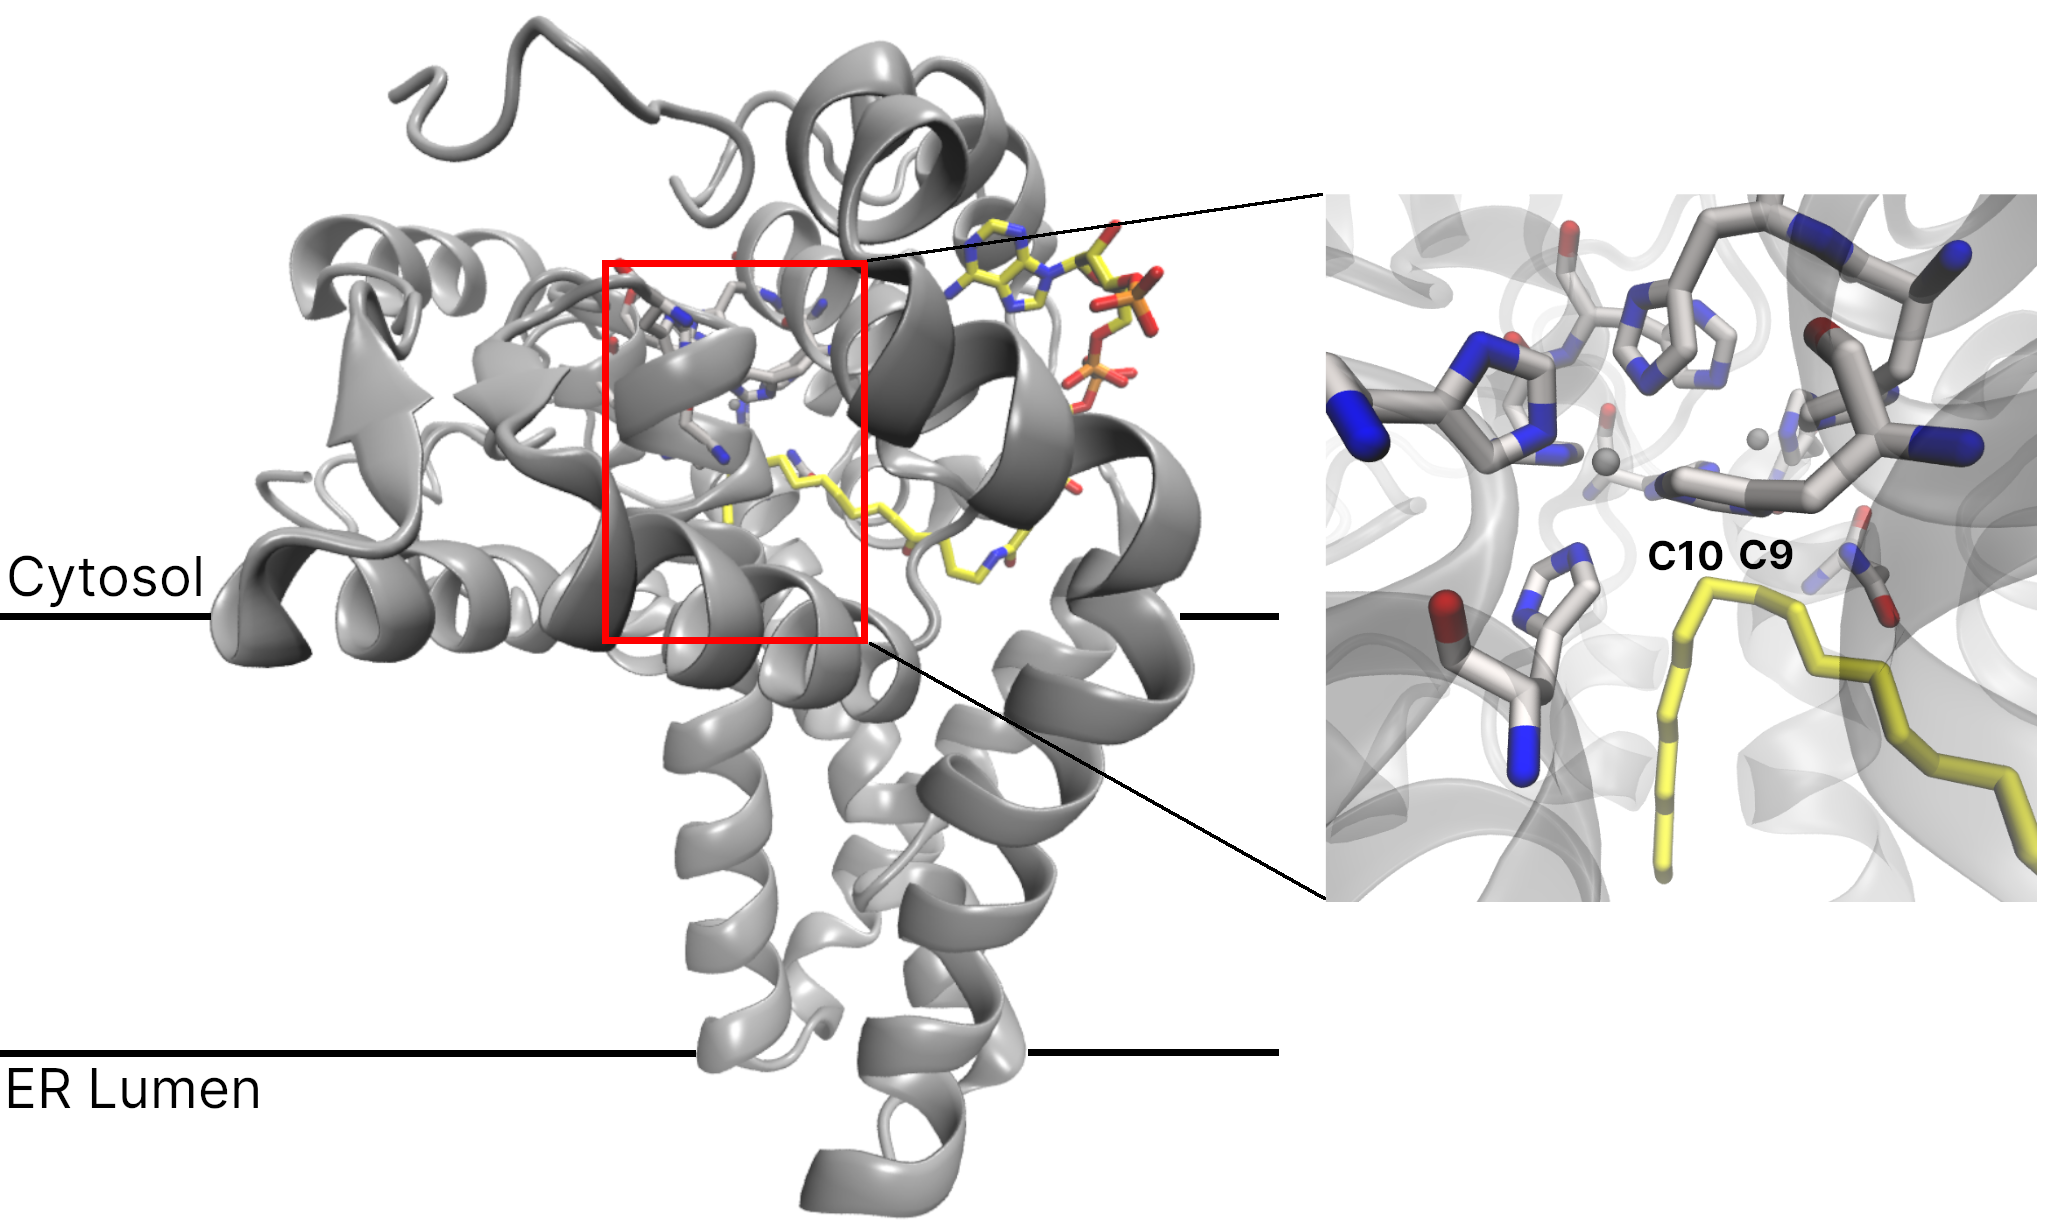
\includegraphics[width=1.0\textwidth]{Figures/SCD1.png}
    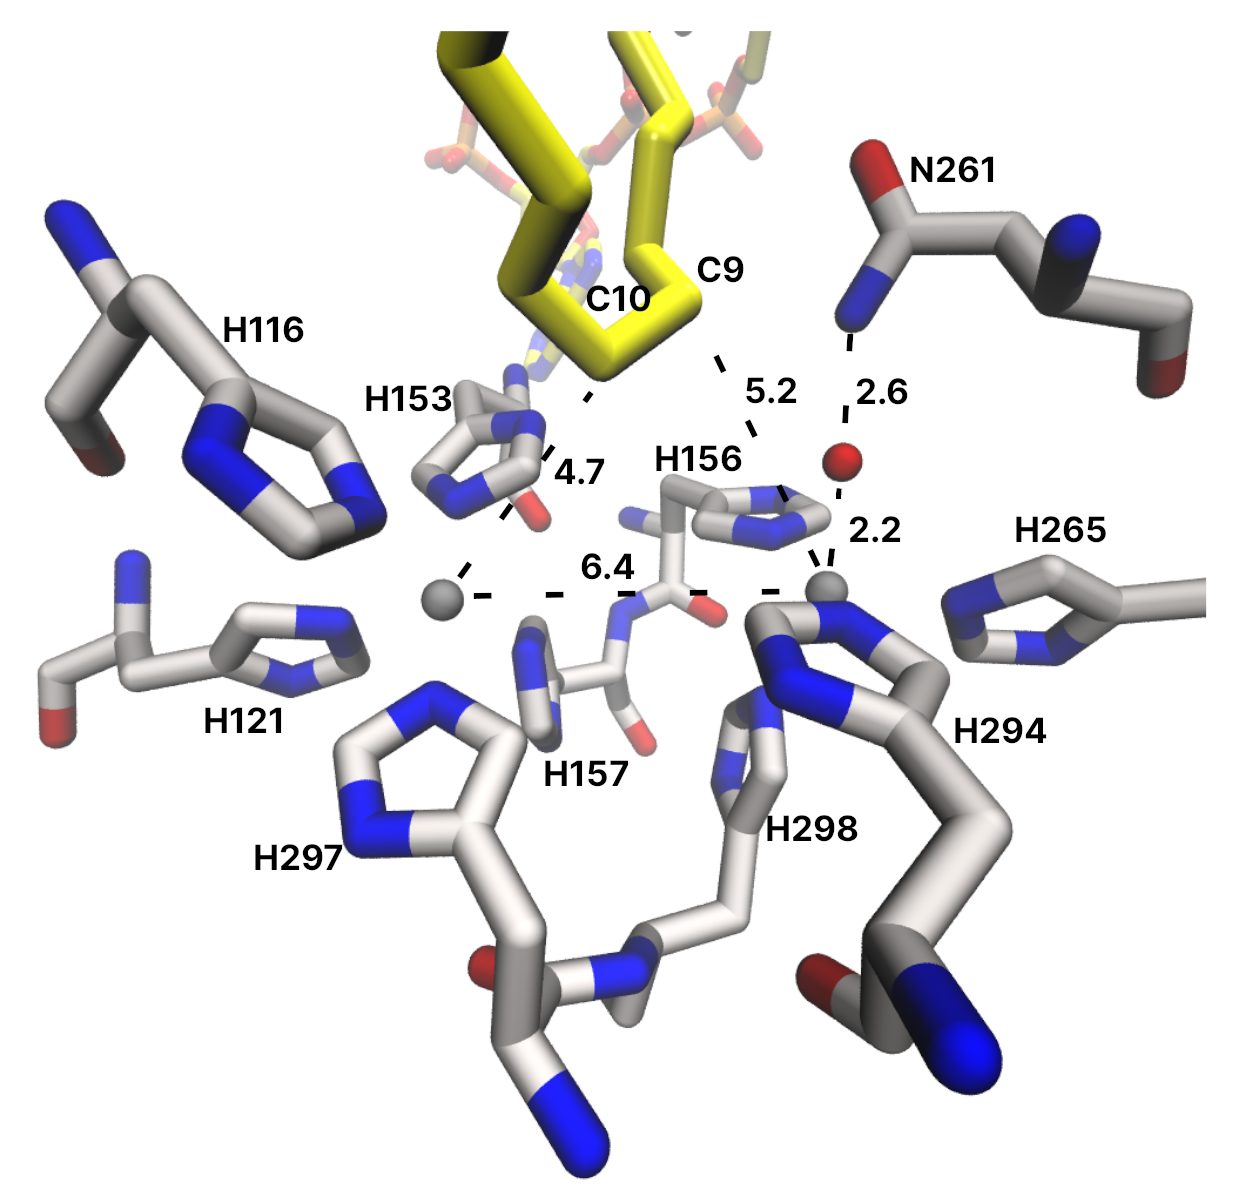
\includegraphics[width=0.7\textwidth]{Figures/scd1_active_site.png}
    \caption{Structure of mouse stearoyl-CoA desaturase in complex with substrate (PDB: 4YMK, \cite{Bai2015}) with a schematic representation of membrane position (top) and geometry of the active site (bottom). Stearoyl-CoA and the active site are shown as sticks. Distances are shown in Å. Colours: silver, zinc; red, oxygen; blue, nitrogen; white, protein carbons; yellow, carbons of stearoyl-CoA and sulfur; orange, phosphorus.}
    \label{fig:SCD1_structure}
\end{figure}


\subsection{Substrate selectivity}
 Enoch et\,al.\,studied the activity of rat SCD1 with acyl-CoA substrates of varying chain lengths \cite{Enoch1976}. SCD1 was active for substrates with aliphatic chains containing between 12 and 19 carbons (Table\,\ref{tab:Enoch_table}). The highest activity is observed for substrates with 17 to 19 carbons. Interestingly, there is a very sharp drop off in activity for eicosanoyl-CoA (20:0). The determined crystal structures offer an explanation of the activity trends \cite{Bai2015}. The short acyl-CoA substrates are not able to reach the turn near the active site, whereas substrates with more than 19 carbons cannot fit into the tunnel. The residues Tyr104 and Ala108 at the end of the tunnel are suggested to limit the maximum chain length. Both residues are highly conserved in animal SCD1. A desaturase from \textit{Calanus hyperboreus} contains a smaller Thr residue in the position of the bulky Tyr104 which possibly explains its preference for long fatty acid substrates (22:0-26:0). Furthermore, mutagenesis studies showed that mutation of Thr to Tyr results in a loss of activity for long chain fatty acids \cite{Meesapyodsuk2014}. Another desaturase from \textit{Drosophilia melanogaster} has a larger Met residue in the position of Ala108 and is only active with fatty acids containing up to 14 carbon atoms \cite{Dallerac2000}.


\subsection{Reaction mechanism}
The desaturation reaction requires the abstraction of two hydrogen atoms, one from C9 and one from C10. This raises the question whether the two HAAs occur simultaneously or in two distinct steps. If the latter is the case, what is the site of initial abstraction? A comparative kinetic isotope effect (KIE) study on SCD1 suggests answers for these questions \cite{Buist1996}. In it, the reaction rate constants are compared for non-deuterated stearoyl-CoA ($k_H$) and for stearoyl-CoA deuterated at C9, and at C10 ($k_D$). The results show a large primary KIE for the C9 deuterated sample (${k_H}/{k_D}\simeq 5-8$) and a very small KIE for the C10 deuterated sample (${k_H}/{k_D}\simeq 1$). This rules out the simultaneous HAA mechanism and suggests initial slow rate-limiting HAA at C9 followed by fast HAA at C10. In support of this mechanism is a study which showed that SCD1 is more efficient at oxidizing the 9-thia analogue of stearoyl-CoA to sulfoxide than the 10-thia analogue \cite{Buist1992}.

SCD1 is a transmembrane binuclear NHFe enzyme and, as was discussed earlier, the identity of the iron-oxygen species responsible for desaturation is not known. Spectroscopic data on AlkB suggests formation of bridged iron-oxygen complexes \cite{Shanklin1997}, but it is not clear if that is possible based on the long iron-iron distance. A cluster model DFT/B3LYP study of the SCD1 active site investigated different possible desaturation mechanisms \cite{Yu2019}. All attempts at finding bridged iron-oxygen species resulted in oxygen binding to just one of the iron ions suggesting a novel oxygen activation mechanism. The full proposed reaction mechanism is shown in figure\,\ref{fig:SCD1_mechanism}. Oxygen binds to the tetracoordinated iron ion (Fe\textsubscript{B}) forming the typical iron(III)-superoxo species (React$_{\alpha}$) which gets transformed to iron(III)-hydroperoxo (Int1$_{\alpha}$, Int2$_{A-\alpha}$). Next, the O$-$O bond breaking is facilitated by hydrogen transfer from a water molecule activated by the other iron ion (Fe\textsubscript{A}) forming a triple-hydroxo intermediate (Int3$_{A-\alpha}$). This is suggested as the rate-limiting step in the proposed mechanism with a barrier of 13.4 kcal/mol. Proton transfer between the two hydroxides on Fe\textsubscript{B} leads to the formation of a high-valent iron(IV)-oxo species (Int4$_{A-\alpha}$) which can abstract the first hydrogen on C9 with a barrier of 10 kcal/mol (Fig.\,\ref{fig:Desaturation}). This is followed by a rapid second HAA from C10 by the hydroxide on Fe\textsubscript{A}. Transfer of an electron regenerates the initial state of the active site. The proposed mechanism is consistent with the KIE results which suggest that HAA on C9 is slow and occurs first. It also provides a nice explanation of the asymmetrical coordination of the iron ions. The tetracoordinated iron needs to have two free coordination positions to accommodate the two groups formed after O$-$O bond breaking while the other iron ion only needs one free position for water activation. Still, more experimental and computational data is necessary to validate the proposed mechanism and there is still the question of how to explain the AlkB spectroscopy data.  

\begin{figure}[htbp]
    \centering
    \includegraphics[width=\textwidth]{Figures/Desaturation_steps.pdf}
    \caption{Hydrogen atom abstraction steps in the proposed mechanism of stearoyl-CoA desaturase. Adapted from \cite{Yu2019}.}
    \label{fig:Desaturation}
\end{figure}

\subsection{SCD1 as a drug target}
Changes in fatty acid metabolism are linked with many diseases. As SCD1 is a key enzyme in fatty acid metabolism, it is a promising drug target. SCD1 inhibitors are studied for the potential treatment of obesity and type two diabetes \cite{Dobrzyn2005}. Studies showed that mice lacking the gene for SCD1 had increased sensitivity to insulin and were resistant to diet-induced obesity \cite{Ntambi2002}. It is suggested that SCD1 deficiency promotes partitioning of fats towards oxidation and in this way protects mice from obesity.

Normal tissue cells usually make use of circulating lipids. Cancer cells, on the other hand, have poor vascularization which results in a higher need for \textit{de novo} lipid synthesis \cite{Ackerman2014}. Membrane lipids are also required to facilitate the rapid growth of cancers \cite{Snaebjornsson2020}. Elevated lipid synthesis was connected to increased tumor growth \cite{Swinnen2006}. Expression of SCD1 was found to be elevated in several human cancer cell lines, including breast cancer \cite{Holder2013}, bladder cancer \cite{Presler2018} and kidney cancer \cite{Wang2015}. The studies also found correlation between higher concentrations of SCD1 and tumor malignancy as well as poorer chances of patient survival.

SCD1 inhibitors indeed show promising results in \textit{in vitro} studies but only few reached clinical testing due to strong side effects \cite{Zhang2014}. Besides the importance in cancer cells, SCD1 is essential for normal functioning of sebum-producing epithelial cells (sebocytes) \cite{Schneider2010}. Sebum is a waxy, oily mixture extracted on the skin, hair and eyes. It reduces evaporation and prevents heat loss. Although mice lacking SCD1 showed resistance to diet-induced obesity \cite{Ntambi2002}, lack of SCD1 also causes severely dry skin and eyes \cite{Miyazaki2001} in addition to hypothermia after exposure to cold \cite{Lee2004}. Tissue specific SCD1 inhibitors do posses better safety properties \cite{Zhang2014}.

Interesting progress in the field was made by Theodoropoulos et\,al.\,who managed to discover tumor-specific irreversible inhibitors of SCD1 \cite{Theodoropoulos2016}. The pro-drug is non-toxic for sebocytes and is selectively activated into an irreversible SCD1 inhibitor in cancer cells by cytochrome P450 (CYP) oxidases. CYPs metabolize drugs and other xenobiotics and are expressed in many cancer cells \cite{Rodriuez2006}. The pro-drug is activated by demethylation exposing a phenol group in the activated drug which irreversibly binds to SCD1, potentially in the diiron active site. The exact binding mechanism is not known but it is suggested to proceed through the formation of phenolic radical species \cite{Winterton2018}. CYPs are also expressed in the liver, but studies on mice showed that SCD1 is not essential in the liver \cite{Miyazaki2007}.


\section{Research goals}
The primary objective of this thesis is to further study the reactive intermediate of SCD1 proposed by Yu and Chen based on a B3LYP cluster model study (Int4$_{A-\alpha}$ from figure \ref{fig:Desaturation}) \cite{Yu2019}. Classical molecular dynamics simulations will be used to explore different conformations of the system. As a prerequisite it will be necessary to prepare the challenging membrane system and develop force field parameters for the metal center. The final goal is to study the intermediate's reactivity with QM/MM molecular dynamics simulations using the semiempirical GFN2-xTB QM method \cite{Bannwarth2019,Bannwarth2020,Grimme2017} combined with higher-level of theory energy corrections. GFN2-xTB showed very good performance in the prediction of the geometry of a diverse set of organometallic transition-metal complexes \cite{Bursch2019}, but to test its performance for the study of the HAA step by Int4$_{A-\alpha}$ a cluster model potential energy surface (PES) scan will be performed and results compared to the reported B3LYP results.

The study will provide a better understanding of the selectivity and reactivity of SCD1 which can help in the design of new inhibitors but also provide insight into the poorly understood mechanism of the whole group of transmembrane NHFe$_2$ enzymes. To the best of our knowledge this will be the first application of multiscale molecular dynamics simulations for the study of reactivity of a transmembrane NHFe$_2$ enzyme. 

